\documentclass[11pt,letterpaper]{article}

% Essential packages
\usepackage[utf8]{inputenc}
\usepackage[T1]{fontenc}
\usepackage[margin=1in]{geometry}
\usepackage{fancyhdr}
\usepackage{graphicx}
\usepackage{float}

% Math packages
\usepackage{amsmath}
\usepackage{amsfonts}
\usepackage{amssymb}
\usepackage{amsthm}

% Table packages
\usepackage{booktabs}
\usepackage{array}
\usepackage{tabularx}
\usepackage{longtable}

% Graphics and plotting
\usepackage{tikz}
\usepackage{pgfplots}
\pgfplotsset{compat=1.18}
\usepackage{subcaption}

% Citation and references
\usepackage[round,authoryear]{natbib}
\usepackage{url}

% Code listings (if needed for simulation code)
\usepackage{listings}
\usepackage{xcolor}

% Hyperlinks (load last)
\usepackage[colorlinks=true,linkcolor=blue,citecolor=blue,urlcolor=blue]{hyperref}

% Custom commands for common actuarial notation
\newcommand{\E}{\mathbb{E}}
\newcommand{\Var}{\text{Var}}
\newcommand{\Cov}{\text{Cov}}
\newcommand{\Prob}{\mathbb{P}}

% Header and footer setup
\pagestyle{fancy}
\fancyhf{}
\fancyhead[L]{Ergodicity Economics in Insurance}
\fancyhead[R]{\thepage}
\fancyfoot[C]{Confidential - Internal Research}

% Title page information
\title{\Large \textbf{Ergodicity Economics in Property \& Casualty Insurance: \\
A Simulation Framework for Understanding Risk Appetite}}

\author{Alex Filiakov, ACAS\\
\texttt{alexfiliakov@gmail.com}}

\date{\today}

\begin{document}

\maketitle

\begin{abstract}
This white paper introduces a new simulation framework based on ergodicity economics principles for analyzing insurance risk appetite in Property \& Casualty markets. Traditional ensemble-based risk models may not adequately capture the temporal dynamics of insurance company decision-making. This introductory paper demonstrates that insurance appetite varies significantly with company size, measured by revenue.

\textbf{Keywords:} ergodicity economics, insurance appetite, risk modeling, simulation framework
\end{abstract}

\newpage
\tableofcontents
\newpage

\section{Executive Summary}

This section should provide a concise overview of the entire paper, typically 1-2 pages covering:
\begin{itemize}
    \item The problem addressed
    \item Your key methodology (simulation framework)
    \item Primary finding about company size and insurance appetite
    \item Practical implications for the industry
\end{itemize}

% TODO: Complete executive summary content

\section{Introduction}

\subsection{Current Challenges in Insurance Appetite Modeling}

Traditional approaches to modeling insurance appetite in P\&C markets face several limitations:
\begin{itemize}
    \item Reliance on ensemble averages rather than temporal sequences
    \item Inadequate consideration of path-dependent effects
    \item Limited incorporation of company-specific factors
\end{itemize}

\subsection{The Promise of Ergodicity Economics}

Ergodicity economics, developed by \citet{peters2019ergodicity}, offers a new perspective on decision-making under uncertainty. Unlike traditional expected utility theory, which focuses on ensemble averages, ergodicity economics emphasizes the importance of time averages and growth rates.

% TODO: Add more detailed introduction content

\section{Theoretical Foundation}

\subsection{Ergodicity vs. Non-Ergodicity in Financial Systems}

A stochastic process is ergodic if its time average equals its ensemble average:
\begin{equation}
\lim_{T \to \infty} \frac{1}{T} \int_0^T f(X_t) dt = \E[f(X)]
\end{equation}

\subsection{Insurance Markets as Non-Ergodic Systems}

Insurance markets exhibit non-ergodic properties due to:
\begin{itemize}
    \item Path-dependent capital accumulation
    \item Regulatory constraints on capital adequacy
    \item Finite time horizons for business decisions
\end{itemize}

\subsection{Mathematical Framework}

Let $W_t$ represent the wealth of an insurance company at time $t$. Under multiplicative dynamics:
\begin{equation}
W_{t+1} = W_t \cdot (1 + r_t)
\end{equation}

where $r_t$ represents the return from underwriting and investment activities.

The growth rate is given by:
\begin{equation}
g = \lim_{t \to \infty} \frac{1}{t} \ln\left(\frac{W_t}{W_0}\right)
\end{equation}

% TODO: Expand theoretical section

\section{Simulation Framework Overview}

\subsection{Architecture and Key Components}

The simulation framework consists of several key modules:

\begin{enumerate}
    \item \textbf{Market Environment Module}: Generates stochastic loss scenarios
    \item \textbf{Company Behavior Module}: Models decision-making processes
    \item \textbf{Capital Dynamics Module}: Tracks financial position over time
    \item \textbf{Risk Appetite Measurement Module}: Quantifies appetite changes
\end{enumerate}

\subsection{Input Parameters and Data Requirements}

\begin{table}[H]
\centering
\caption{Key Input Parameters}
\begin{tabular}{@{}lll@{}}
\toprule
Parameter & Description & Source \\
\midrule
Initial Capital & Starting surplus position & Company financials \\
Loss Distribution & Frequency and severity models & Historical data \\
Investment Returns & Portfolio yield assumptions & Market data \\
Regulatory Ratios & Minimum capital requirements & Regulatory filings \\
\bottomrule
\end{tabular}
\end{table}

\subsection{Model Validation and Calibration}

% TODO: Describe validation methodology

\subsection{Computational Considerations}

The simulation employs Monte Carlo methods with:
\begin{itemize}
    \item 10,000 simulation paths per scenario
    \item 20-year projection horizons
    \item Quarterly decision points
\end{itemize}

\section{Case Study: Company Size and Insurance Appetite}

\subsection{Methodology and Assumptions}

Our primary hypothesis is that insurance appetite, defined as the willingness to underwrite additional risk, varies systematically with company size.

Key assumptions:
\begin{itemize}
    \item Companies maximize long-term growth rates rather than expected utility
    \item Risk appetite is measured by the Kelly criterion adaptation for insurance
    \item Company size is proxied by annual revenue
\end{itemize}

\subsection{Data Sources and Parameterization}

% TODO: Describe data sources and parameter estimation

\subsection{Results Presentation and Interpretation}

\begin{figure}[H]
\centering
% TODO: Add actual simulation results plot
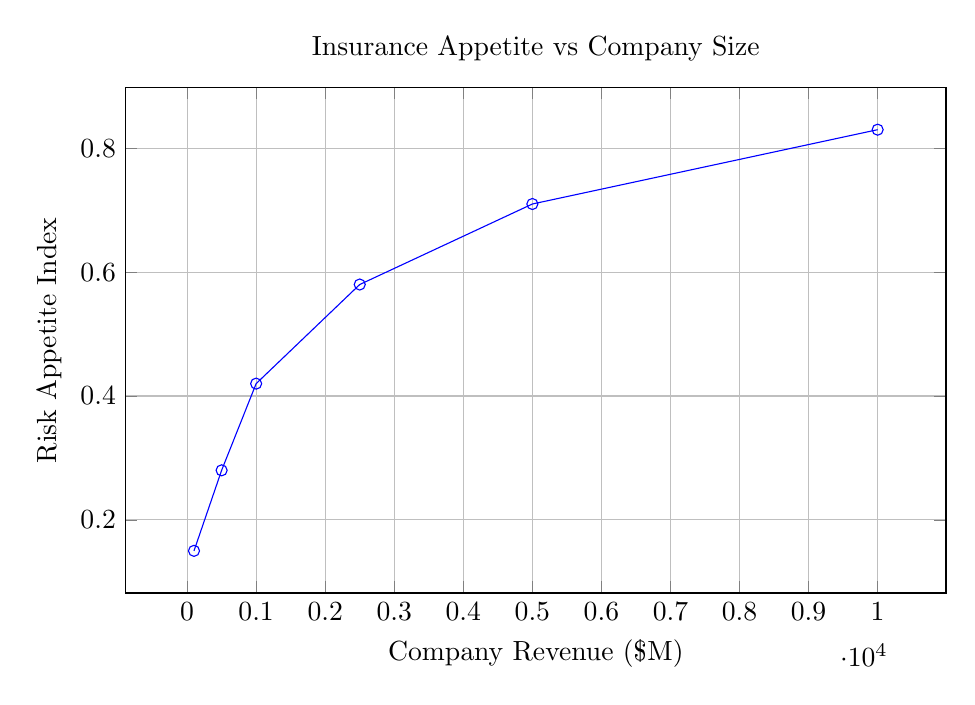
\begin{tikzpicture}
\begin{axis}[
    xlabel={Company Revenue (\$M)},
    ylabel={Risk Appetite Index},
    title={Insurance Appetite vs Company Size},
    grid=major,
    width=12cm,
    height=8cm
]
% Placeholder data - replace with actual results
\addplot[blue, mark=o] coordinates {
    (100, 0.15)
    (500, 0.28)
    (1000, 0.42)
    (2500, 0.58)
    (5000, 0.71)
    (10000, 0.83)
};
\end{axis}
\end{tikzpicture}
\caption{Risk appetite increases with company size (simulated results)}
\label{fig:appetite_vs_size}
\end{figure}

Figure \ref{fig:appetite_vs_size} demonstrates the positive correlation between company size and risk appetite, consistent with ergodicity economics predictions.

\subsection{Sensitivity Analysis}

% TODO: Present sensitivity analysis results

\section{Industry Implications}

\subsection{Applications for Underwriting and Pricing}

The simulation framework provides several practical applications:
\begin{itemize}
    \item Dynamic pricing models that account for company size effects
    \item Portfolio optimization considering temporal risk dynamics
    \item Competitive positioning analysis
\end{itemize}

\subsection{Portfolio Management Considerations}

% TODO: Discuss portfolio management implications

\subsection{Regulatory and Capital Allocation Insights}

% TODO: Discuss regulatory implications

\section{Future Research Directions}

\subsection{Framework Extensions and Enhancements}

Potential areas for future development include:
\begin{itemize}
    \item Integration with catastrophe modeling
    \item Multi-line portfolio effects
    \item Reinsurance optimization
\end{itemize}

\subsection{Additional Applications in P\&C Insurance}

% TODO: Outline future applications

\subsection{Industry Collaboration Opportunities}

% TODO: Discuss collaboration possibilities

\section{Conclusion}

This white paper has introduced a novel simulation framework based on ergodicity economics principles for analyzing insurance risk appetite. Our key findings demonstrate that company size significantly influences risk appetite, with larger insurers exhibiting greater willingness to underwrite risk. This finding has important implications for competitive dynamics and market structure in P\&C insurance.

The simulation framework provides a powerful tool for:
\begin{itemize}
    \item Understanding temporal risk dynamics
    \item Optimizing portfolio decisions
    \item Informing strategic planning
\end{itemize}

I encourage industry practitioners to explore these concepts further and welcome collaboration on extending this research.

The framework will provide new insights for companies making insurance decisions and is intended to answer questions such as "what is the ROI of our insurance program?", "how much insurance do we need?" and considerations of optimal insurance deductibles and limits.

% Bibliography
\bibliographystyle{apalike}
\bibliography{references}

% Appendix
\appendix
\section{Technical Appendix}

\subsection{Simulation Algorithm Details}

% TODO: Provide detailed algorithm descriptions

\subsection{Parameter Estimation Methods}

% TODO: Describe statistical methods used

\subsection{Code Repository}

The simulation framework code is available at: \url{https://github.com/your-repo/ergodicity-insurance}

\end{document}
